% Project 2 - EECS 499
% Author: Shaun Howard (smh150@case.edu)
\documentclass[conference]{IEEEtran} \usepackage[T1]{fontenc} \usepackage[backend=biber, style=ieee]{biblatex}
\addbibresource{report.bib} \usepackage[final]{microtype}

% graphics
\ifCLASSINFOpdf \usepackage[pdftex]{graphicx} % declare the path(s) where your graphic files are
  \graphicspath{{images/}} % and their extensions so you won't have to specify these with
  % every instance of \includegraphics
  \DeclareGraphicsExtensions{.jpeg,.png} \else
\fi


\begin{document}

\title{Jacobian Pseudo-inverse RRT Path Planner with Randomized-IK Restarts for Baxter Dual Arm Manipulator}

\author{
 \IEEEauthorblockN{Shaun Howard}
 \IEEEauthorblockA{Electrical Engineering and Computer Science Department\\
                   Case Western Reserve University\\ 
                   Cleveland, Ohio 44106\\
                   Email: smh150@case.edu}
}

% make the title area
\maketitle

% As a general rule, do not put math, special symbols or citations
% in the abstract
\begin{abstract}
Within this paper a flexible solution to the path planning problem for dual-arm robots is presented. Several methods are implemented for path planning with the 
Jacobian transpose and pseudo-inverse, using various forms of gradient descent. The construction of an Randomly RRT is presented which plans with the Jacobian 
pseudo-inverse for goal-directed movement and randomly restarts with a randomly-selected Inverse Kinematics solution point near the goal to avoid getting stuck 
in local minima. Several variations on the algorithm are tested, including switching between the Jacobian transpose and pseudo-inverse to compare planning 
accuracy, efficiency, and speed between the two gradient descent methods. The test results for the four algorithm combinations are compared. The results have 
yielded the focus of the paper to be on the pseudo-inverse gradient descent method for motion planning with random IK restarts for the Baxter dual arm 
manipulator.
\end{abstract}

\section{Introduction} \label{Introduction}

The search for accurate and quick planning algorithms has grown in recent years with major breakthroughs in memory architecture, processing unit speed and 
parallel processing. Several planning methods exist that were slow and infeasible to do in real-time in the past. These algorithms can now be resurrected and 
reused successfully on modern hardware. The planner described in this paper is a versatile planner that has several options for planning. The first option is to 
use only the Jacobian Transpose for planning. The algorithm for the RRT-JT from <paper1> influenced the JT planner implemented in this paper.  While this 
method's computational time is small and plans are accurate, it's planning capabilities are somewhat limited. The Jacobian Pseudo-inverse (JPI) adds yet more 
versatility to the planner by itself. The JPI planner utilized in this paper was influenced by multiple sources, primarily <paper2>. This method was also found 
to be a bit slow in descending to the goal. A method was implemented to increase the speed of descent as described in <paper3>. The implementation of this method 
allowed the planner to have two more variations, including the JT with speedup and JPI with speedup. 

A test bed was built for testing these algorithms with the Gazebo simulator, Rviz, and the Microsoft Xbox Kinect for Point Cloud environment visualization. An 
obstacle avoidance collision checker was added to detect obstacles and plan in avoidance of them during RRT construction. While experimenting with RRT 
construction, the nodes were found quick enough to unravel from the normal RRT construction pattern. The pattern is to create the entire tree and prune nodes, 
then to execute the path. That type of planning assumes a static environment that does not change during RRT construction. The planner framework presented in 
this paper updates obstacles upon each available update in an asynchronous fashion. This functionality is provided by creating a new ROS node that solely updates 
Kinect obstacle clouds for the robot to subscribe to with a ROS subscriber.

The Baxter robot has two 7 degree of freedom (DOF) arms. A multi-threaded extension was added to the planner to plan for both arms simultaneously and checking 
for obstacle collisions when validating solutions, while dynamically creating and executing RRT nodes on the robot. The obstacle collision checker filters 
each arm from its own obstacle cloud when possible. This allows each arm to plan in accordance for the other arm, to avoid collisions. Most of the experiments 
with the planner described in this paper isolate each arm from the other for testing accuracy and speed on complex goal poses. Poses ranging from easy to 
complex are tested and compared. The Jacobian PINV method paired with random IK restarts turned out to be the most effective and efficient method for motion 
planning with both arms as it is multi-threaded and modern computational power provides fast computation for the JPI.

The works related to the planner described in this paper are outlined in the next section. Following, the problem for dual-arm motion planning is established. 
After that, sensor measurements and capturing data with the Kinect setup are discussed. Later, the implementation is discussed along with experimentation and 
simulator set up. Second to last, experimentation results are analysed and compared. Lastly, the paper is concluded with the results of the experiments.

\begin{figure}
\label{pic1} 
\centering 
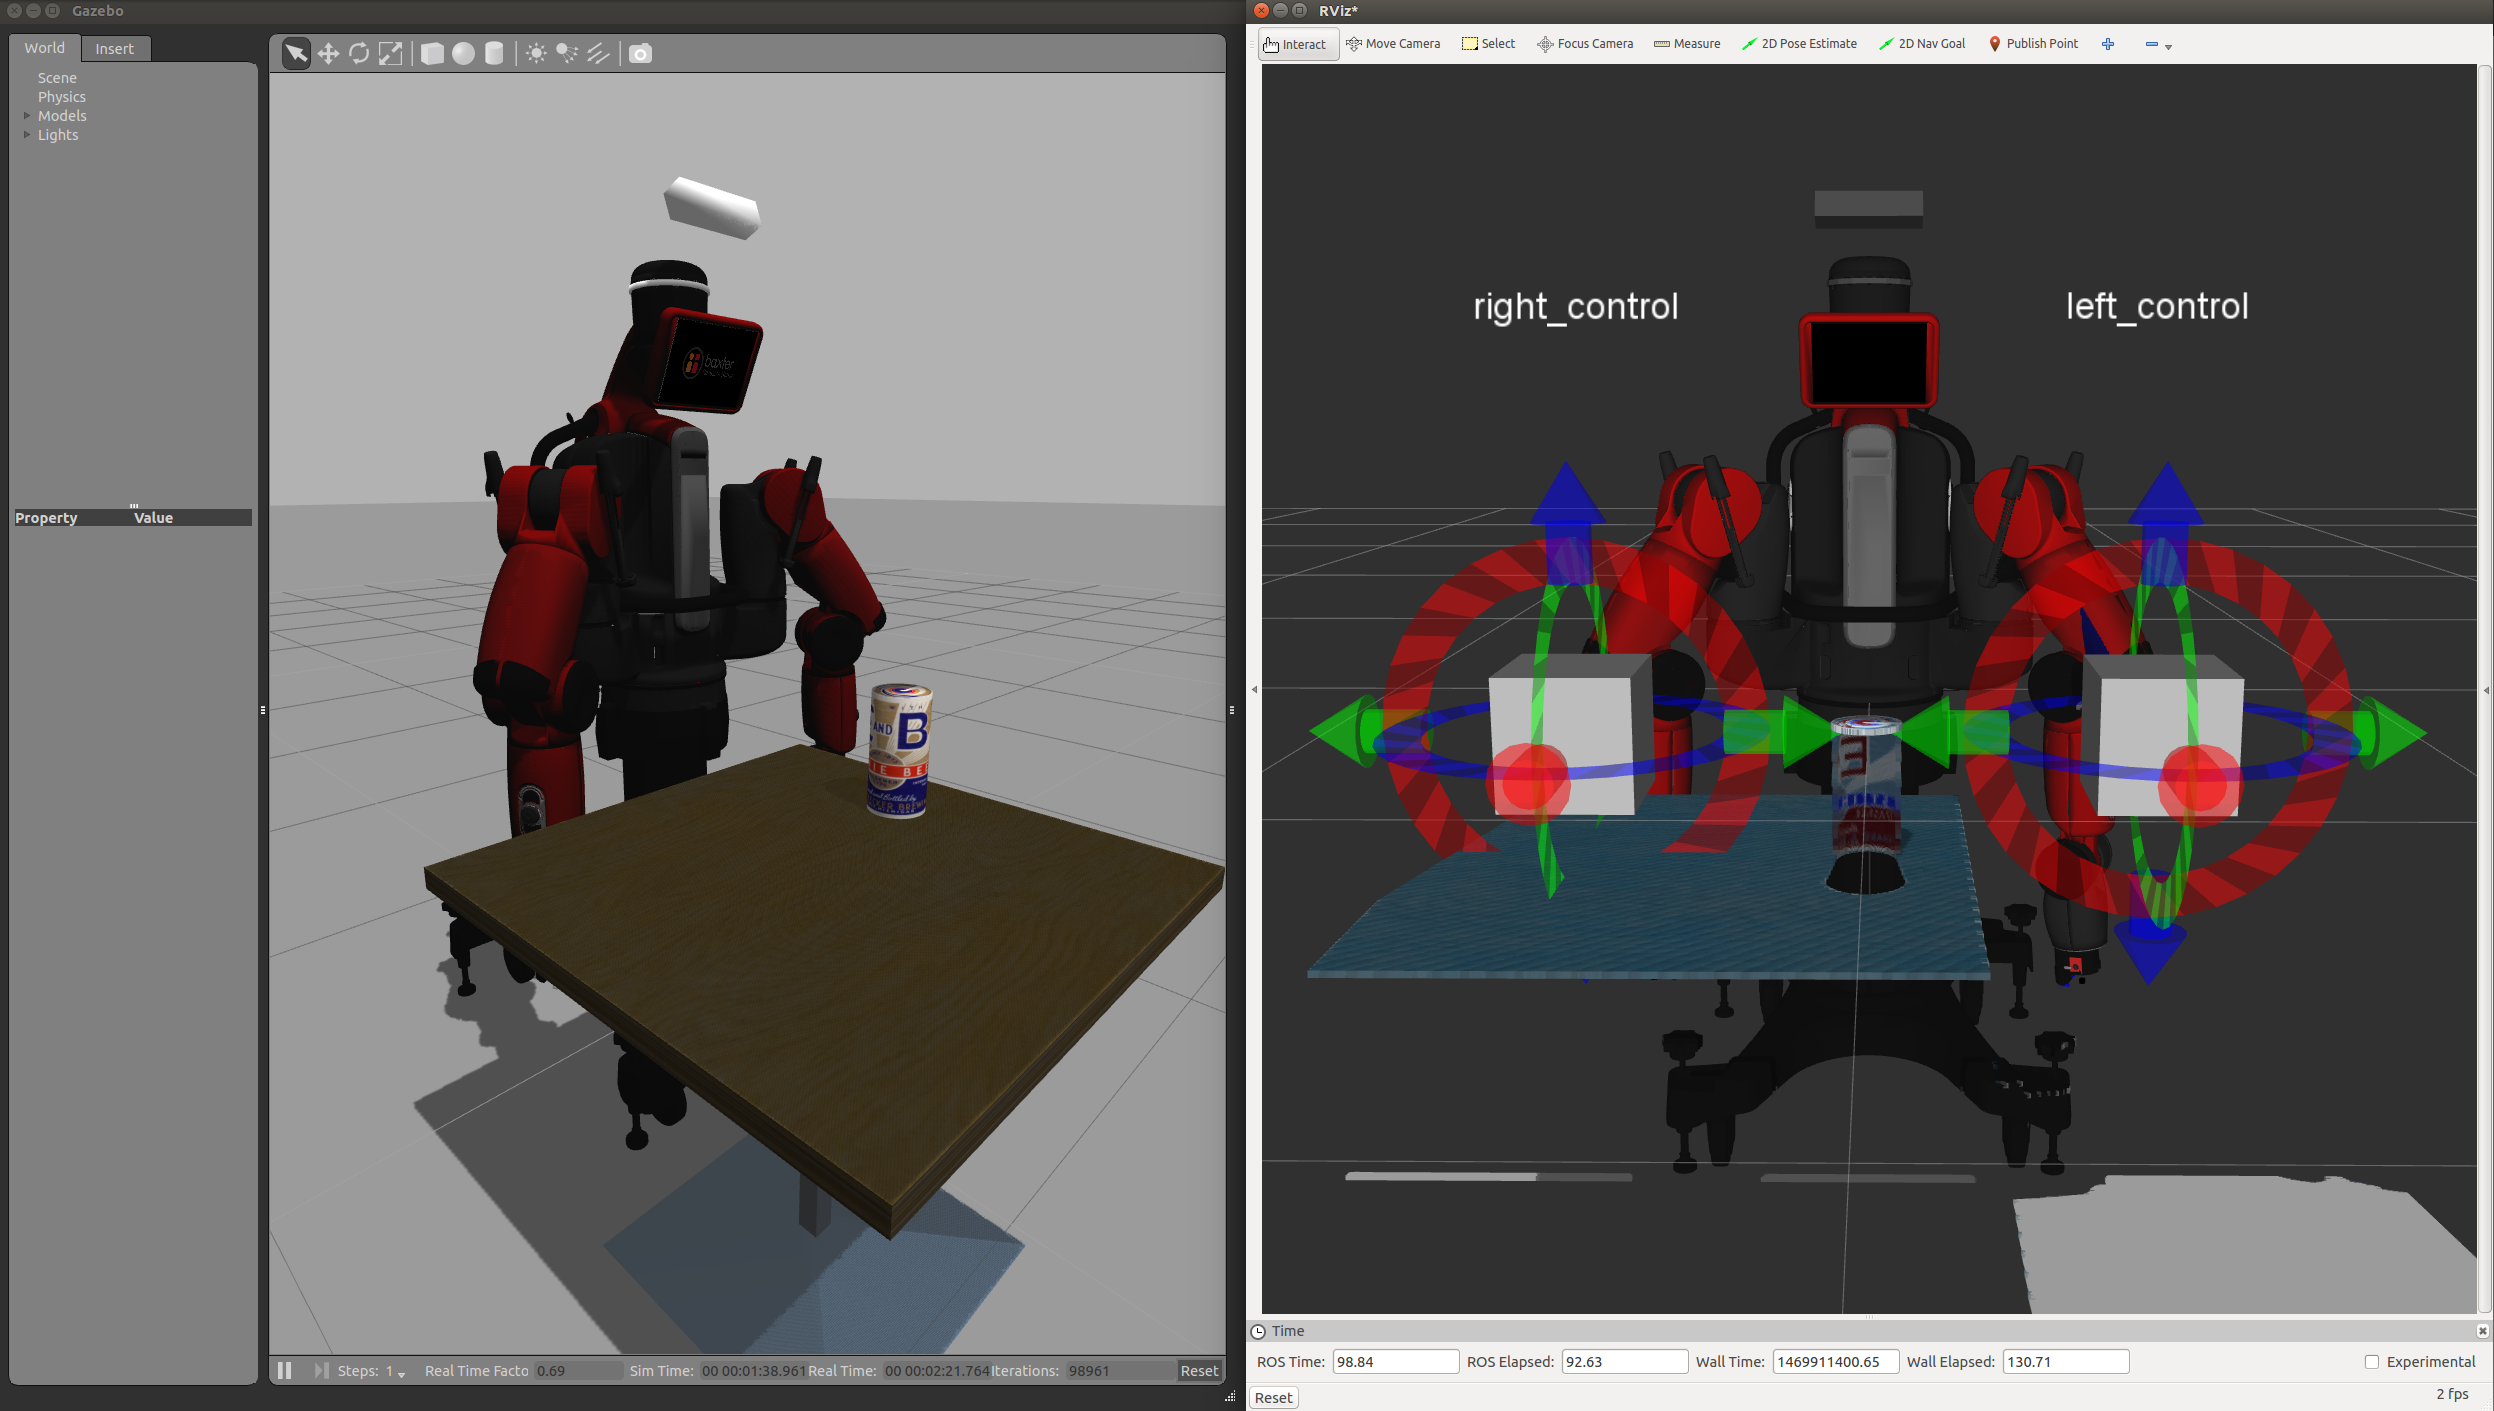
\includegraphics[width=0.49\textwidth]{sim1}
\caption{The Baxter simulator set-up with the Microsoft Xbox Kinect and some objects useful for obstacle detection in the scene.}
\end{figure}

\section{Related Work} \label{Related Work}

The first planner method used to implement the baseline planner was the RRT-JT, as implemented in \cite{random_planner_wo_ik}. This method was useful for getting the 
robot moving and setting up a groundwork for accuracy and performance. The paper combines the idea of an RRT with the usage of a goal-directed modification to 
the typical RRT algorithm, causing the end effector to approach the goal in a direction leading it closer to the goal than previous RRT methods. Another valuable 
aspect of this planner method is that it does not rely at all on IK solvers. The true pitch for this method is to be used in systems where IK solutions are hard 
or cost-ineffective to find.

The second planner method that the JPINV is based on is described in \cite{humanoid_motion_planning}. This paper focuses on diverse outlooks to the RRT-JT planner and 
make new additions with the PINV and IK methods. They also feature dual-arm planning algorithms that plan for both arms simultaneously. Their paper outlines a 
modern framework of comparison for arm motion planning techniques that has provided this research with a sensible baseline for this planner using random PINV and 
IK solutions.

The third planner method is pioneered in the workspace goal region paper \cite{wgr_planning}. The paper utilizes concepts from \cite{humanoid_motion_planning} to 
holistically solve the obstacle avoidance problem for motion planning. Workspace goal regions (WGR) are areas that the arm can operate in safely and efficiently. 
Outlying area is either inefficient or an impossible point to reach to say the least. The more advanced gradient descent method used to improve upon the first 
two planning methods is outlined in this paper. The method speeds up descent to local minima while the randomness is still at play in the planner because they 
apply the RRT-JT method.  

The fourth planner method was just discovered as an additional way to apply the JPINV method with the sped up gradient descent. The JT is switched with the 
JPINV and the planner improves in performance and accuracy. \cite{humanoid_motion_planning} inspired the use of the PINV in replacement of the transpose for this 
planning variation.

\section{Problem Formulation} \label{Problem Formulation}

The problem of motion planning for humanoid robots with high degrees-of-freedom has been an ongoing area in robotics. The search for a faster, more responsive
planning system with high accuracy is a hard one. The problem is that most planners assume a static environment and assume the robot has a large amount of time
to determine a solution for a grasp. RRT planners typically take tens of seconds to solve solutions, but they do not move the robot until the path is complete.
There ends up being a long turnaround time for some plans and other plans are impossible to execute due to joint limits and other workspace constraints.

The JT addition to the typical RRT construct provides a goal-directed approach to motion planning, rather than an exhaustive random search. This allows the
planner to reach the goal in a shorter amount of time, making the RRT planning method more useful for real-time applications. The problem with the RRT-JT 
approach is that joint limits are met fairly quickly. The descent approach used in this process also takes quite an amount of time to converge to the solution 
since the JT steps are small. \cite{humanoid_motion_planning} discusses the weaknesses of the JT method, including those mentioned.

The PINV method was introduced in \cite{humanoid_motion_planning}. The problem with typical RRT planners is that they are single-threaded, so the entire solution 
requires that the environment be static, neither arm moves, and the solution cannot be executed until both arms are planned for synchronously. Since real-
time demands have grown for modern robots, single-threaded planning methods are out-dated and almost unusable. Given the previous speed of RRT
construction, planning for multiple arms would be a hassle and very time-intensive process, making dual arm planning inefficient in modern environments.

One of the main problems with the PINV method besides computation time is the ability to easily get stuck in local minima while planning. Since the JPINV method draws
the solution to the goal very quickly, there is little time to compensate for the large step size of the PINV method without solving a very hard problem. Fortunately,
as discovered in \cite{wgr_planning}, there is some matrix math that alleviates the issue of controlling the gradient direction and magnitude without much complexity. 
The planning algorithms presented in \cite{wgr_planning} are much more applicable for modern systems in terms of computing accuracy, utilizing a static workspace 
region with minimum and maximum values that the arm can plan for solutions within, but this is actually a drawback for dynamic environments in most realistic humanoid 
robot-oriented environments. Thus, some improvements must be made to this method for real-time collision avoidance support. This solution is not presented in a 
generalized fashion for multiple arms, thus the performance of the solution has yet to be analysed in synchronous or asynchronous computation between two or more 7-
dof arms. It can be assumed that running this planner synchronously for two or more limbs would be very difficult and time consuming. 

Overall, the solutions to most of these problems include the application of multi-threading and asynchronous updates, separating methods that are computationally 
intensive or rely on time series data into their own nodes or threads in a program.

\section{Methodology} \label{Methodology}

The planner needs to solve the problems presented in the problem formulation section. Most of the problems stem from hardware requirements, lack of parallel processing and 
lack of real-time updates about environment obstacles and goal regions. The planner designed in this paper must parallelize the computationally intensive methods into 
their own nodes or processing threads in the program for the robot. The first objective in the planner is to observe and avoid obstacles. The capture and filtering of data is covered in the next subsection.

\subsection{Sensor Measurements} \label{Sensor Measurements}

The Microsoft Xbox Kinect is used to collect point cloud data about the robot environment in the experiments. The point clouds are red-green-blue-depth (RGB-D) clouds. 
Thus, the color and depth information can be read and processed for filtering out points from the clouds to do pre-processing steps on them before they reach the robot. 
The points are received in the kinect\_pc\_frame, however almost all planning algorithms are based on goal poses in the robot base frame. Thus, the points must be 
transformed from the kinect\_pc\_frame to the base frame in order to make any sense to the robot's planners. Following, the immediate workspace cloud is constructed of 
points filtered above a certain z-position, since Baxter's arms cannot quite reach the floor on any usual base. The points can easily be filtered in x,y,z minimum and 
maximum ranges. The point of such filtering is to speed up image processing and obstacle detection time, thus in turn speeding up planning time as well. Each arm is 
considered it's own unit of execution, thus it will have it's own thread. each arm has different obstacle regions than the other to avoid because one arm is the obstacle
of another arm. Thus, it is useful for each arm to have it's own filtered obstacle cloud. 

The left arm's obstacle cloud should have the left arm filtered out. The right arm's obstacle cloud should thus have the right arm filtered out of it. If these obstacle
clouds are updated frequently and the planner can update its obstacle regions for each arm to plan with on-demand, then this method of filtering is a part of the solution
to the problem of real-time planning in dynamic environments that the papers described thus far have lacked. The idea to do real-time updates stems from experimentation
with the RRT. The RRT-JT implementation already appears that it can be de-coupled from the usual complete tree-building RRT solution before execution and be executed on a 
per-node basis by the end effector while planning is still happening to reach the goal. The thought of this de-coupling brings in the concept of a time series data model, 
where obstacle clouds are updated at each possible time step and the planner will receive and update itself with the latest obstacles over time with planning. Thus, the 
solutions are based on random samples, will never be the same again and are unpredictable, but this provides a solid foundation for speed of the RRT-JT solver, since
it is goal-directed and guaranteed to converge unless the goal is unreachable or would exceed goal limits.

The idea of updating obstacles asynchronously, on-demand provides the ability to parallelize arm-planning and speed up the entire process tremendously. This idea also 
allows data sharing between planner threads for most of the pre-processed workspace points, saving computational space, time and work. Not only did previous papers lack 
the ability of asynchronously updating obstacles, but they treated the environment statically during RRT construction. In modern applications, a static environment
assumption would crumble the foundation of the RRT solution, especially since RRTs can be slow for more complex trajectories and goal poses. The planners in this paper 
will have a hook to the asynchronous obstacle updates and will receive the latest filtered obstacle clouds for their arm in order to provide the concept of real-time 
motion planning with real-time obstacle avoidance to the extent of the speed of the point cloud unpacking, updating, transformation and filtering operations on the 
hundreds of thousands of four-dimensional RGB-D data points.
 
\subsection{Planner Design}

The planner design in this paper is inspired by all of the best qualities of the planners described in the papers mentioned. Modifications were made to the concept of a Rapidly-
exploring Random Tree necessary to fuse the several successful Jacobian-based techniques together to provide reliable redundant manipulator planning. This hybrid 
RRT planner provides the ability to use either the Jacobian-Transpose or Jacobian Pseudo-inverse-based methods for goal-directed path planning. For random path planning, a IK
straight-line solver is used to sample solutions at random points within growing radii from the goal center until a goal is found or the maximum number of retires is met. 
The pairing of the hybrid RRT and random IK-based planner methods should allow solutions to be found very quickly if possible, otherwise, the planner should get as close as 
possible to the goal over time or once a goal distance threshold is met. 

The planner framework consists of four different options for planning, using either the JT or JPINV as an error measurement technique. The surrounding planner structure was built
purposefully for versatility and adherence to a specific planner interface that could be generalized for several arms. Given the Baxter robot has 2 arms, the version of
the planner for this paper has two arms -- both the left and right arms -- implemented in a multi-threaded fashion to increase planner turnaround time and provide a 
sense of real-time planning for modern humanoid robot applications. The planner considers all obstacles for each arm at frequently updated time steps and executes new
nodes once they are verified as collision free and within a certain range from the goal. Several parameters exist in the planner that can be tweaked to make it
perform better such as the allowed range to the goal. Currently, default settings have been set to ensure optimal performance for experimentation purposes.
The planner details including pseudo-code to the RRT-JT and RRT-JPINV paired with random IK restarts as well as parameters that can be tuned will be covered in the 
next section.

\subsection{RRT-JT with Random IK Restarts}

The inspiration for random IK restarts with the RRT-JT planner came from the idea of stochastic processes. The RRT-JT planner can get stuck in local minima or reach joint
limits like most other Jacobian-based planners. A great addition to undermine the predetermined nature of getting stuck in minima for the planner would be to add random
restarts somehow. One of the more convenient and reliable ways of doing so would be to add random IK restarts. These random IK restarts would not be sampled from a database,
but points would be randomly generated in a range increasing over time with execution. The benefit of doing so would be that the planner would always be able to climb out of local
minima during gradient descent due to the randomness of the RRT random extend step which is uniformly-selected with a probability of 1-p_goal, where p_goal is the probability 
of the planner extending to the goal with either the JT or JPINV algorithms. As infants experiment with things until they get the answer they
want about why something happens as in cause and effect, the planner would randomly guess when randomly extending to a node with the random-point IK solver would be a good idea.
An addition to this would be to have a set of heuristics to determine when to switch planners for planner turnaround minimization. However, currently, a the probability
p_goal is the deciding factor to switch between the random extension step and the goal extension step of the planner.

The following is pseudo-code for the RRT-JT with random IK restarts:

\subsection{RRT-JPINV with Random IK Restarts}


inspiration: realtime rrt, learning by doing


\subsection{Planner Implementation} \label{Planner Implementation}

\subsection{Gazebo Simulation} \label{Gazebo Simulation}
 A Gazebo simulation paired with Rviz is used to examine custom implementations of the algorithms mentioned. 
 
\section{Results} \label{Results}
A comparison is made between the methods used 
during experimentation which reveals that the hybrid RRT planner is quicker than the other planning methods while balancing constraints and generating a viable solution to 
almost any problem within reach of the given end effector in use.

\section{Conclusion} \label{Conclusion} 
This method was found to perform better than the Jacobian-Transpose and IK-based approaches overall, although 
each method has upsides and downsides. Rarely, if ever, does the planner get noticeably stuck in local minima unless a goal is impossible for the end effector to 
reach.

\subsection{Future Work}

\printbibliography
\end{document}